\section{Configuration}

\subsection{Question P1}
% TODO Préparez un schéma de câblage et d’adressage de votre infrastructure
\begin{figure}[H]
	\centering
	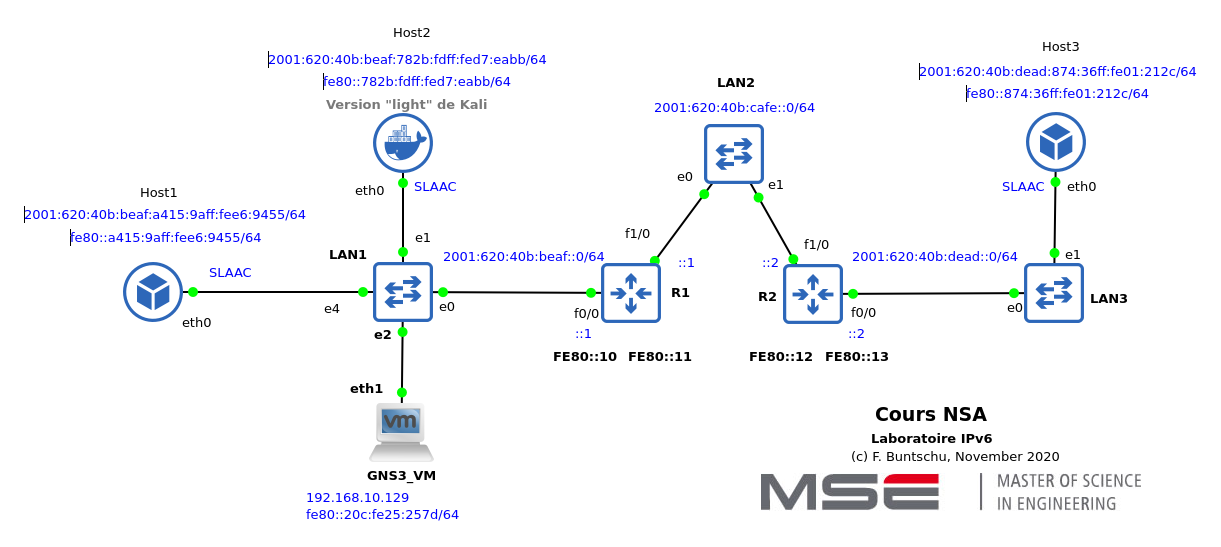
\includegraphics[width=\linewidth]{images/gns_ipv6s.png}
	\caption{Scheme of the all network}
	\label{fig:gns_network}
\end{figure}

\subsection{Question P2}
% TODO Validez que la connectivité IPv6 est fonctionnelle en affichant les tables de routages (show ipv6 route)

\inputminted{text}{files/P2_ipv6_Routers_tables.txt}
\Caption{output of show ipv6 route}
\label{conf:ips_routers}

\subsection{Question P3}
% TODO Quelles sont les adresses IPv6 que les stations ont obtenues ? Commentez
 Every device receives 2 different ipv6 addresses:
\paragraph{scope global dynamic mngtmpaddr} represents the equivalent of ipv4 public address and it is routable on the internet. \textit{Global addresses start with 2001}
\paragraph{scope link} is meant to be used inside an internal network and they are not routed on the Internet. \textit{Link local addresses start with fe80}

\inputminted{text}{files/P3_H1_ipv6_addresses.txt}
\Caption{IPs of host1}
\label{conf:ips_H1}

\inputminted{text}{files/P3_H2_ipv6_addresses.txt}
\Caption{IPs of host2}
\label{conf:ips_H2}

\inputminted{text}{files/P3_H3_ipv6_addresses.txt}
\Caption{IPs of host3}
\label{conf:ips_H3}

\subsection{Question P4}
% TODO Quels types de messages ICMPv6 mesurez-vous ? Quel est leur utilité ?
Using wireshark it is possible to see that nearly every 160 seconds a \Lcode{Router Advertisment} message is send from the router to the device. Following \href{https://www.cisco.com/assets/sol/sb/RV320_Emulators/RV320_Emulator_v1.0.1.01/help/DHCP7.html}{the maunual page} this type of messages are used by the host for learning the prefixes and parameters for the local network.

\begin{figure}[H]
	\centering
	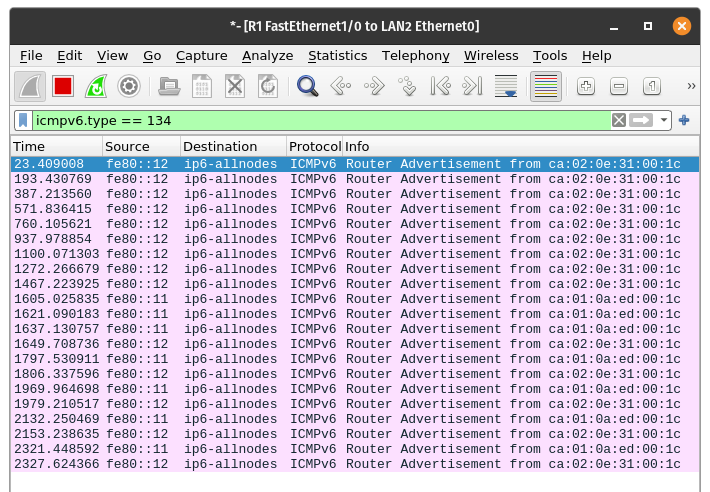
\includegraphics[width=0.8\linewidth]{images/P4_ICMPv6_R_adv_croped.png}
	\caption{ICMPv6 messages: Router Advertisement}
	\label{fig:router_advertisement}
\end{figure}


\subsection{Question P5}
% TODO Est-ce que le Host 1 peut communiquer avec le Host 3 ? Quelles adresses utilisez-vous pour cette communication ?
The host 1 is able to ping the host 3 by using its global address with the following command \scom{ping6 2001:620:40b:dead:874:36ff:fe01:212c} 

\begin{figure}[H]
	\centering
	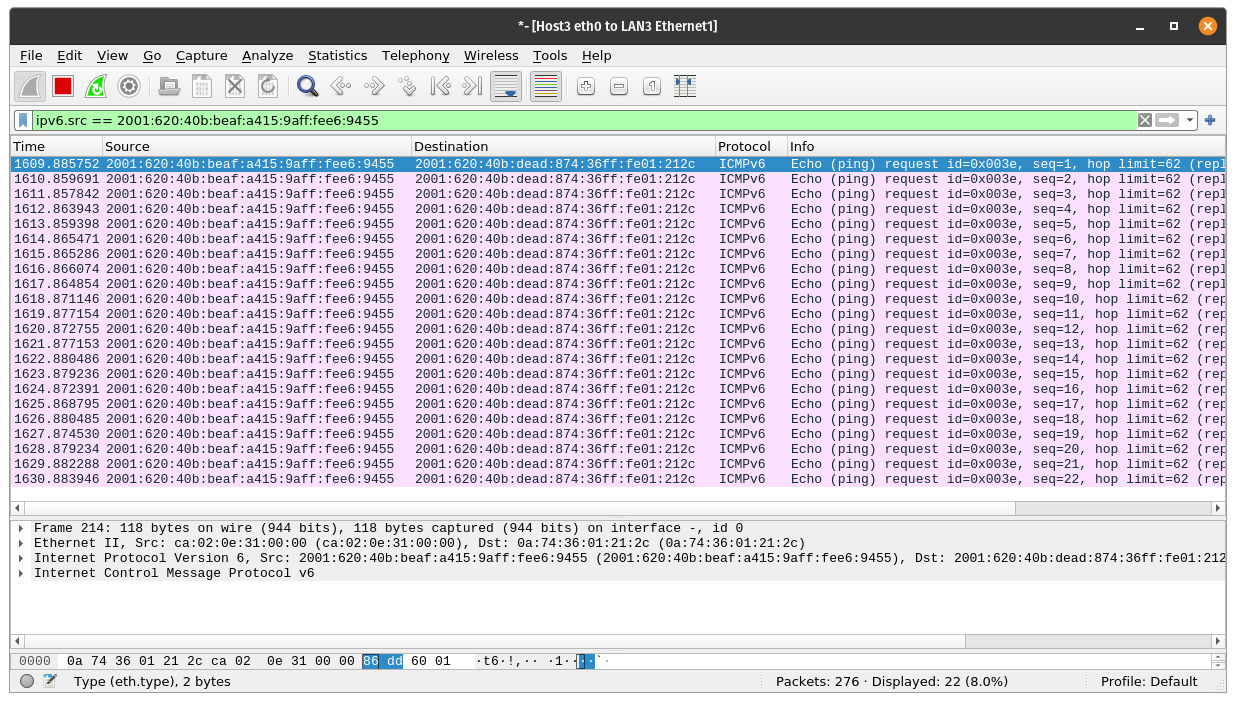
\includegraphics[width=0.8\linewidth]{images/P5_H1_to_H5.png}
	\caption{IPv6 global ping}
	\label{fig:ping_H1_H3}
\end{figure}

\subsection{Question P6}
% TODO Veuillez utiliser ces différents outils et repérer tous les éléments IPv6 de votre infrastructure. Documentez les options utilisées et les résultats obtenus.
In order to get information on the network infrastructure a combination of the command \Lcode{ping6} and \Lcode{ip neighbor}. The idea behind is to send an ICMPv6 echo request message to the all-nodes multicast address. Doing so all nodes that were listening sent back the ICMPv6 echo reply message. When these received these messages, their link-local (and MAC) addresses were added to our neighbor cache.
The full commands entered in the Host 2 command line are: \scom{ping6 -I eth0 -I 2001:620:40b:beaf:782b:fdff:fed7:eabb ff02::1} \scom{ip neighbor}
The obtained results are:

\inputminted{text}{files/P6_neighbor_cache.txt}
\Caption{ping6 and ip neighbor}
\label{log:ping6_neighboor}

Using the command \scom{atk6-passive\_discovery6 eth0} only the local ipv6 of the router 1 could be detected from the host 2.

\subsection{Question P7}
% TODO Quels sont les autres outils que vous avez à disposition pour effectuer cette reconnaissance ? Comment fonctionnent-ils ?

In order to get all information of the network some other tools can be used. For example, \Lcode{traceroute}. With the following command: \scom{traceroute <destination ipv6>} 
entered in the shell of Host 1 the following result has been returned:

\inputminted{text}{files/P7_traceroute.txt}
\Caption{traceroute H1 - H3}
\label{conf:traceroute_H1_H3}

Thanks to this command all the IPs of the machines between the H1 and H3.

Another useful command for getting information on the network is \Lcode{netstat}. If tested in the Host 3 the following output is registered

\inputminted{text}{files/P7_netstat.txt}
\Caption{netstat H3}
\label{conf:netstat_H3}

\subsection{Question P8}
% TODO Quelles sont les informations que vous trouvez dans le Neighbor Cache de vos machines Linux/Windows et ceux des routeurs ?
Here are reported the contents of all neighbor caches:
\inputminted{text}{files/P8_neighbor_chache.txt}
\Caption{Neighbor cache}
\label{log:neighbor_chache}

\subsection{Question P9}
% TODO Quel(s) est(sont) la(les) contre-mesure(s) possible(s) pour palier à la cartographie du réseau en IPv6 ?
In order to prevent the complete cartography of the network some protections of the ICMPv6 protocol can be added. One of the options used is SeND (Secure Network Discovery) employ cryptographically generated addresses (CGA) to encrypt NDP messages. This method is independent of IPSec, which is typically used to secure IPv6 transmissions. The introduction of CGA helps to nullify neighbor/solicitation/advertisement spoofing, neighbor unreachability detection failure, DOS attacks, router solicitation, and advertisement and replay attacks.

\subsection{Question P10}
% TODO Quels sont les effets de cette attaque sur le routeur R1 et sur le Host 1 ?
Thanks to this kind of attacks the gateway is cleaned from the default gateways by the hacker who send a Router Advertisement with a liftime very small to the attacked host. This means that the host has lost the GW. In order to do this attack using the tool THC the following command must be entered in Host 2 \scom{atk6-flood\_router26 -s eth0}

Figure \ref{fig:router26_H1_R1} is the capture taken of the moment of the attack an it is visible that the Router lifetime is set to 1 second when in the default Router Advertisement is set to 1800 seconds.

\begin{figure}[H]
	\centering
	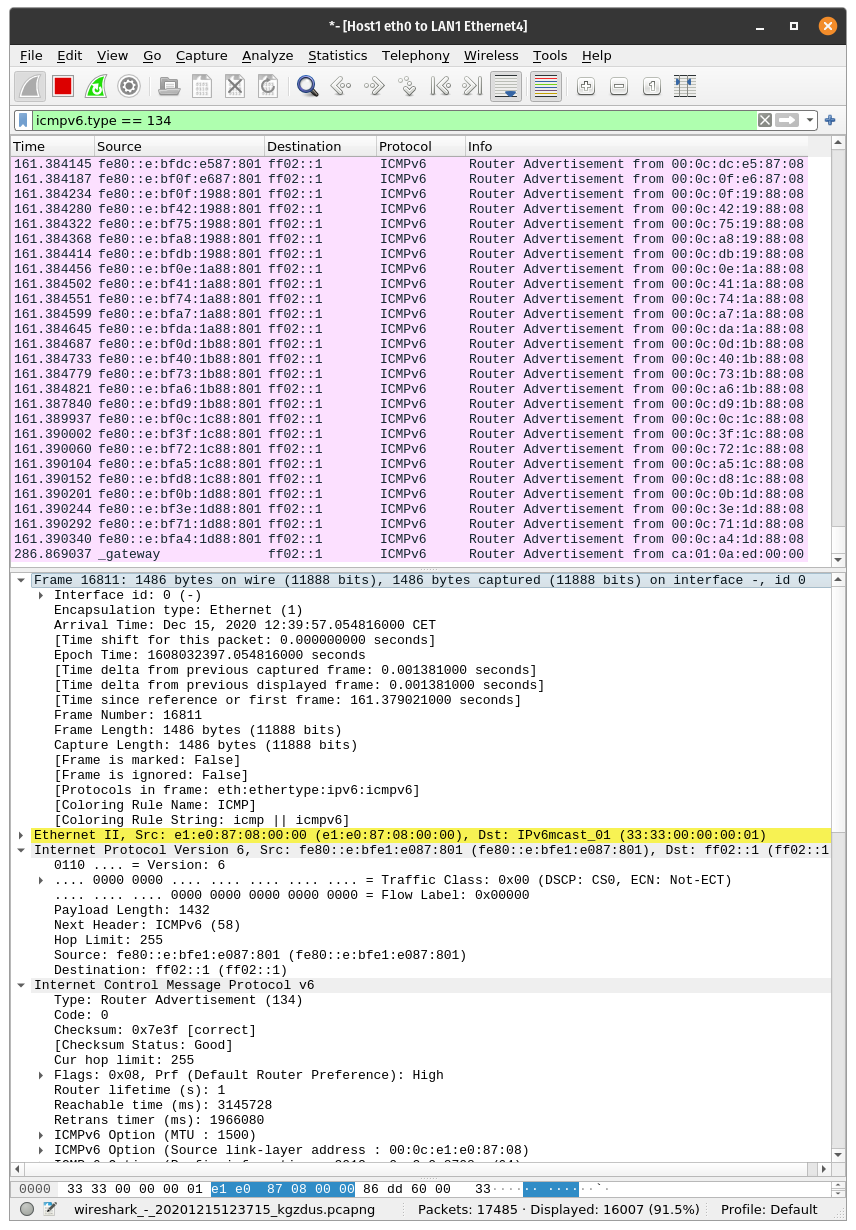
\includegraphics[width=\linewidth]{images/P10_SLAAC_DoS.png}
	\caption{Wireshark capture H1 and R1}
	\label{fig:router26_H1_R1}
\end{figure}

In order to verify that the attack was successful the neighbor cache has been checked resulting in more than 1000 lines reporting:

\inputminted{text}{files/P10_ip_neighbor.txt}
\Caption{Neighbor cache after the attack}
\label{log:P10_neighbor_chache}


\subsection{Question P11}
% TODO Quel(s) est(sont) la(les) contre-mesure(s) possible(s) ?
 In order to prevent this kind of attacks the use of SeND as well as a RA-Guard can be useful.

\subsection{Question P12}
% TODO Où positionnez-vous l’attaquant ?
The hacker needs to be in the same LAN and in the configuration described in figure \ref{fig:gns_network}, if Host 1 is the victim then Host 2 is the attacker.

\subsection{Question P13}
% TODO Décrivez votre configuration, votre attaque et les résultats obtenus.

The configuration used is the same of the previous attack, where the Host 2 is the attacker and Host 1 is the victim. 

The attack started when on the Host 2 the following command has been entered:

Immediately, using a capture of the line between the Host 2 and the LAN1 sw a burst of Router Advertisement messages has been send from the Host 2 to redirect the traffic to it self. During the period of the attack some of the ping messages form the Host 1 have been effectively redirected to the Host 2 (capture \ref{fig:deviated_ping}). In this picture it is visible that some part of the generated traffic has been send to the false destination.

\begin{figure}[H]
	\centering
	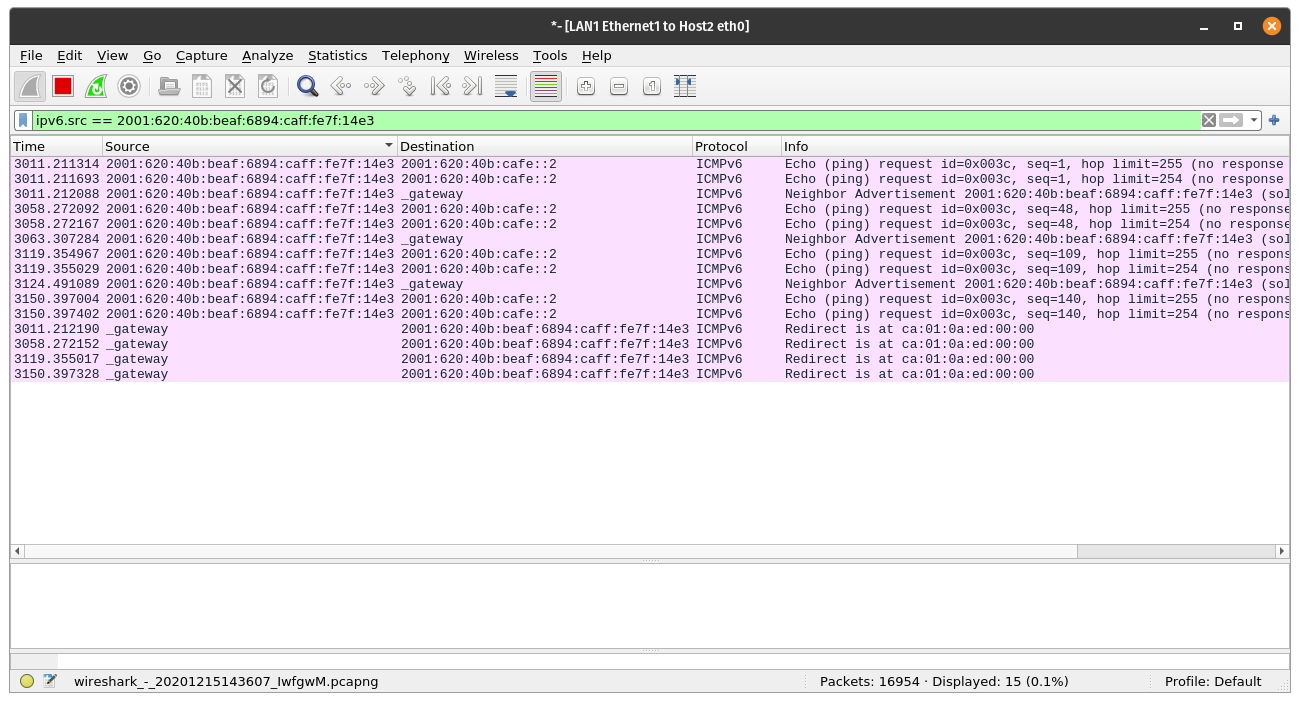
\includegraphics[width=\linewidth]{images/P13_deviated_ping.png}
	\caption{Wireshark capture LAN1 - H2}
	\label{fig:deviated_ping}
\end{figure}
 
Note: during the first try of the attack the host 1 had to be rebooted resulting in having a new global ip address that has been used to continue with the TP \Lcode{2001:620:40b:beaf:6894:caff:fe7f:14e3/64} 

\subsection{Question P14}
% TODO Voyez-vous les requêtes et les réponses ? Pourquoi ?
During the attac not all the traffic has been redirected towards the Host 2 resulting in a partial but nevertheless interesting attack. The following image is a capture done while both the attack and the ping were in action.

\begin{figure}[H]
	\centering
	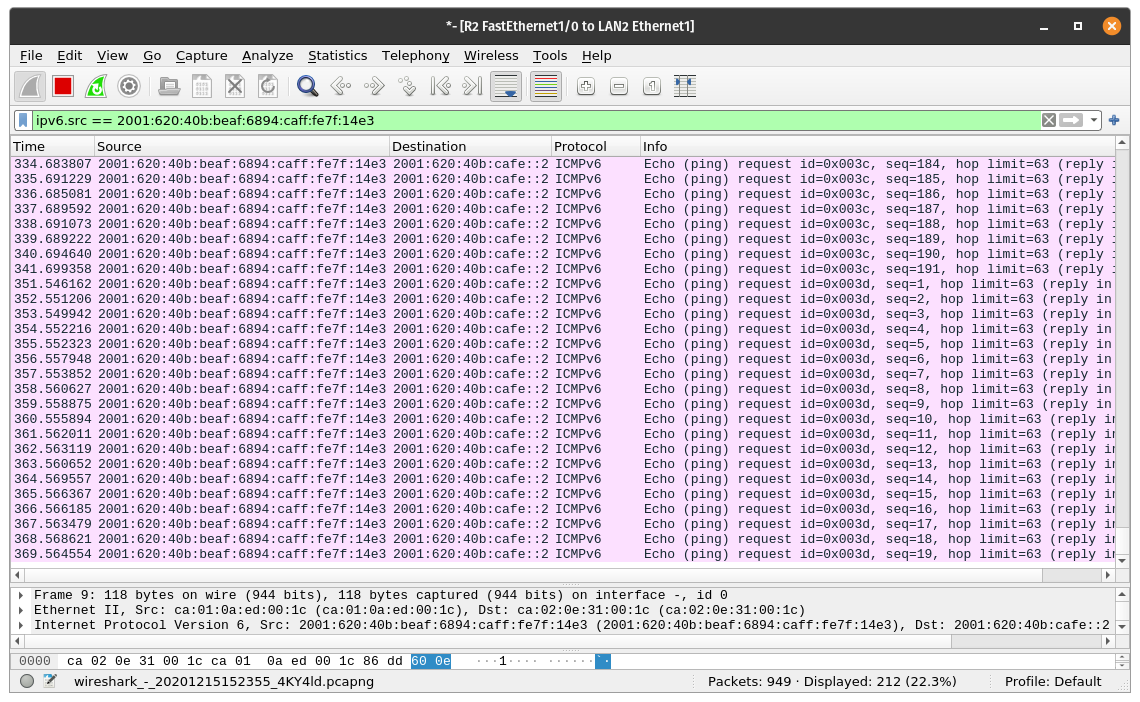
\includegraphics[width=\linewidth]{images/P14_H1_R2.png}
	\caption{Wireshark capture H1 - R2}
	\label{fig:not_deviated_ping}
\end{figure}

\subsection{Question P15}
% TODO Quel(s) est(sont) la(les) contre-mesure(s) possible(s) ?
The possible counter measures are "ad hoc roules" in the SW configuration. RA-Guard is an effective way of controlling this attack and preventing them. The use of SeND is as well a good alternative.

\subsection{Question P16}
% TODO Décrivez cette attaque (fonctionnement et effet)
During this attack the attacker sends lots of RA messages each time with a different prefix. This way the attacked Host 1 creates lot of different IPs. This results in the Host 1 "thinking" to be connected to a multitude of different networks. In the log \ref{log:P16_before_flood} are reported the IPs that Host 1 had before the attack and il log \ref{log:P16_after_flood} the result of a very brief attack is already very visible. In the images \ref{fig:P16_H1_LAN2} and \ref{fig:P16_H2_LAN1} two wireshark captures are reported for showing the burst of RA send from the Host 2 during the attack.

\inputminted{text}{files/P16_before_flood.txt}
\Caption{IPs of Host 1 before the attack}
\label{log:P16_before_flood}

\inputminted{text}{files/P16_after_flood.txt}
\Caption{IPs of Host 1 after the attack}
\label{log:P16_after_flood}

\begin{figure}[H]
	\centering
	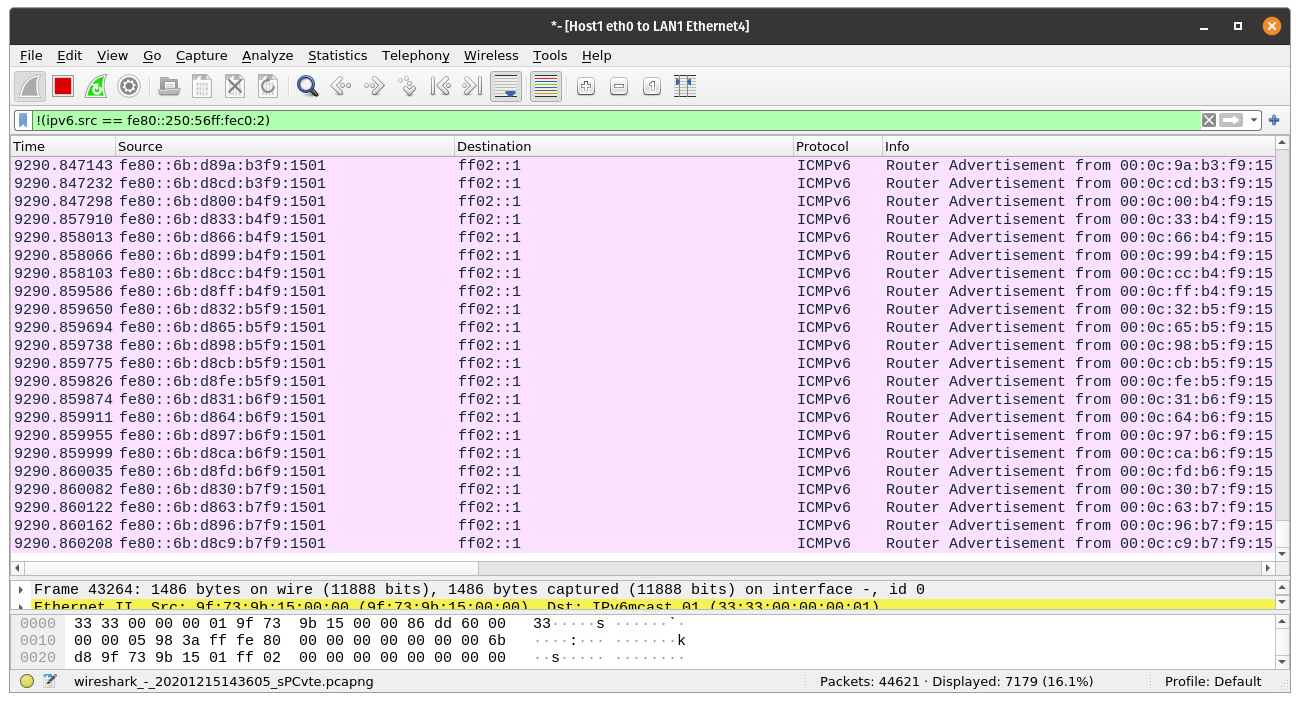
\includegraphics[width=\linewidth]{images/P16_H1_LAN2.png}
	\caption{Wireshark capture H1 - LAN1}
	\label{fig:P16_H1_LAN2}
\end{figure}

\begin{figure}[H]
	\centering
	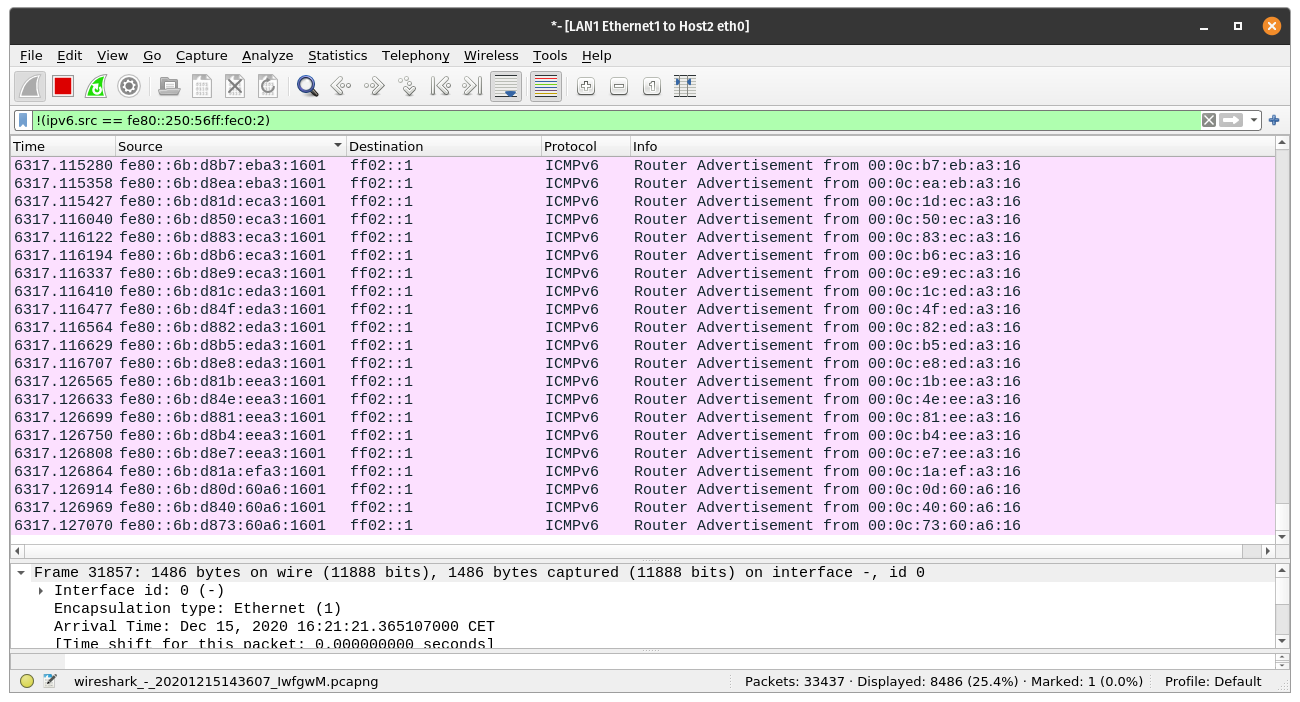
\includegraphics[width=\linewidth]{images/P16_H2_LAN1.png}
	\caption{Wireshark capture H2 - LAN1}
	\label{fig:P16_H2_LAN1}
\end{figure}

\subsection{Question P17}
% TODO Quel(s) est (sont) le(s) impact(s) de cette attaque sur les routeurs R1 et R2 ?


\subsection{Question P18}
% TODO Quel(s) est (sont) la(les) contre-mesure(s) possible(s) ?
A very effective way of preventing a similar attack is the one of filtering the RA using a mechanism of RA-Guard as it was suggested for the previous attacks and as well the use of SeND. Another way of preventing this kind of malicious attacks is to isolate the different Hosts on separated VLANs.

\subsection{Question P19}
% TODO Donnez la liste des outils disponibles et leur utilité (fonctionnement et effets).
Here the tools with their description:
\inputminted{text}{files/P19_THC_toolkit.txt}
\Caption{THC tool}
\label{log:thc_tool}

\href{https://manpages.debian.org/testing/thc-ipv6/index.html}{Manual page}

\subsection{Question P20}
% TODO Décrivez cette attaque (fonctionnement et effets).
How is reported in the manual page of the THC tool the command \Lcode{parasite6}, how it can be easily deduced from the name,is: \begin{quotation} an "ARP spoofer" for IPv6, redirecting all local traffic to your own system (or nirvana if fake-mac does not exist) by answering falsely to Neighbor Solitication requests.
\end{quotation}


The log of the parasite6 command has been the following and it is visible its correspondence with the wireshark captures (\ref{fig:P20_H1_LAN2} and \ref{fig:P20_H2_LAN1}).

\inputminted{text}{files/P20_parasite_log.txt}
\Caption{Log of the attack with parasite}
\label{log:parasite6}
 
During this attack all packages have been spoofed from the attacker and this is visible by performing a ping from the Host 1 and the R2. In the following images it is visible that the traffic is redirected.
\begin{figure}[H]
	\centering
	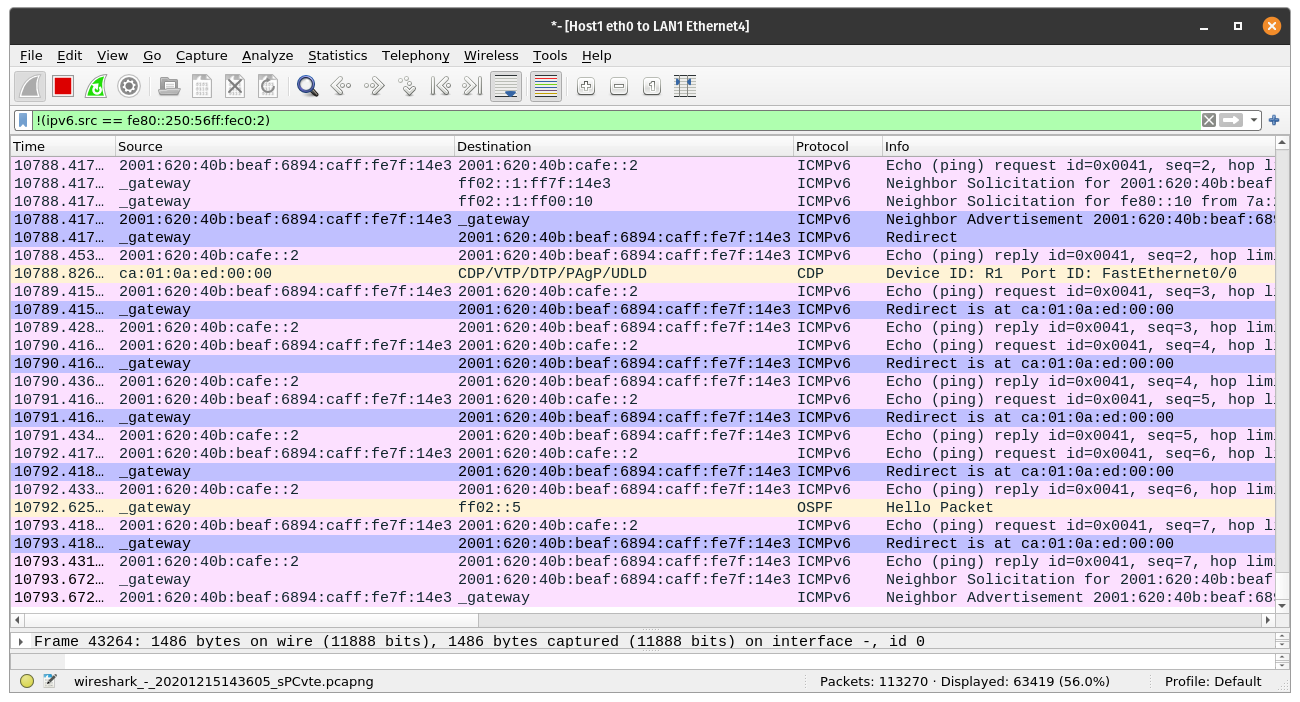
\includegraphics[width=\linewidth]{images/P20_1.png}
	\caption{Wireshark capture H1 - LAN1}
	\label{fig:P20_H1_LAN2}
\end{figure}

\begin{figure}[H]
	\centering
	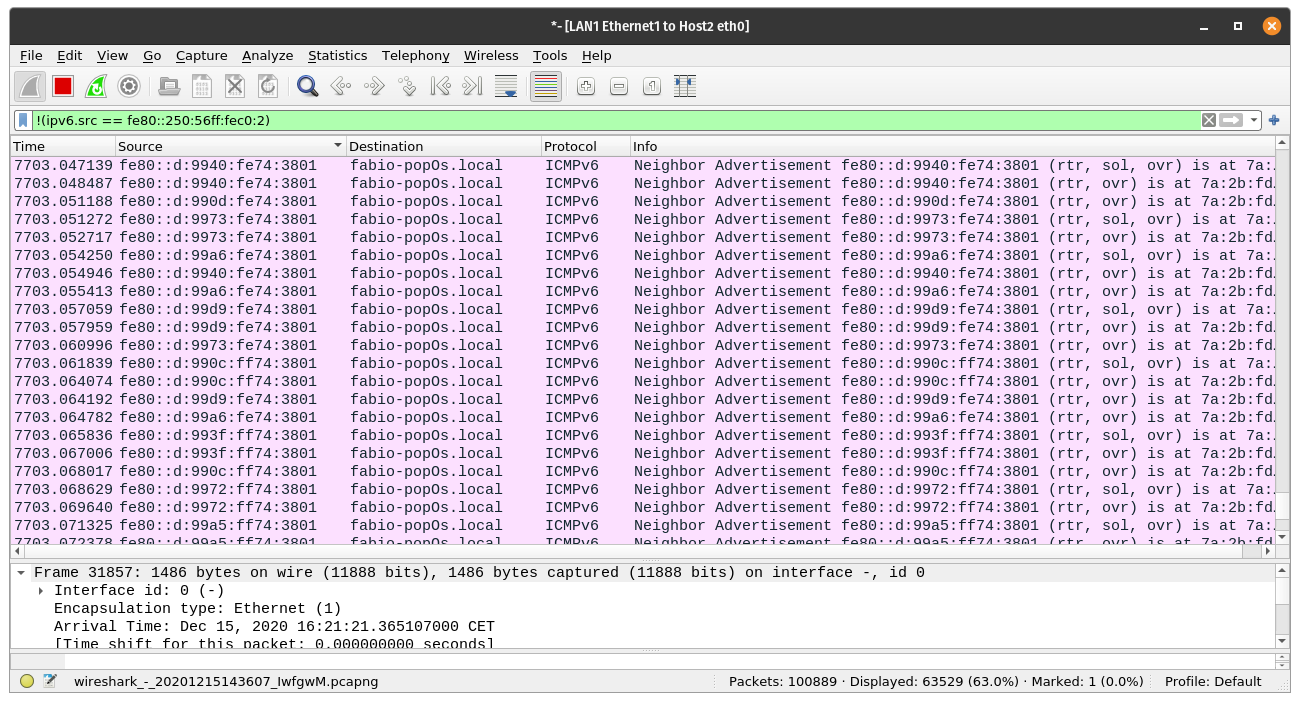
\includegraphics[width=\linewidth]{images/P20_2.png}
	\caption{Wireshark capture H2 - LAN1}
	\label{fig:P20_H2_LAN1}
\end{figure}
